\documentclass{standalone}
\usepackage{tikz}
\usetikzlibrary{patterns, positioning}


\begin{document}
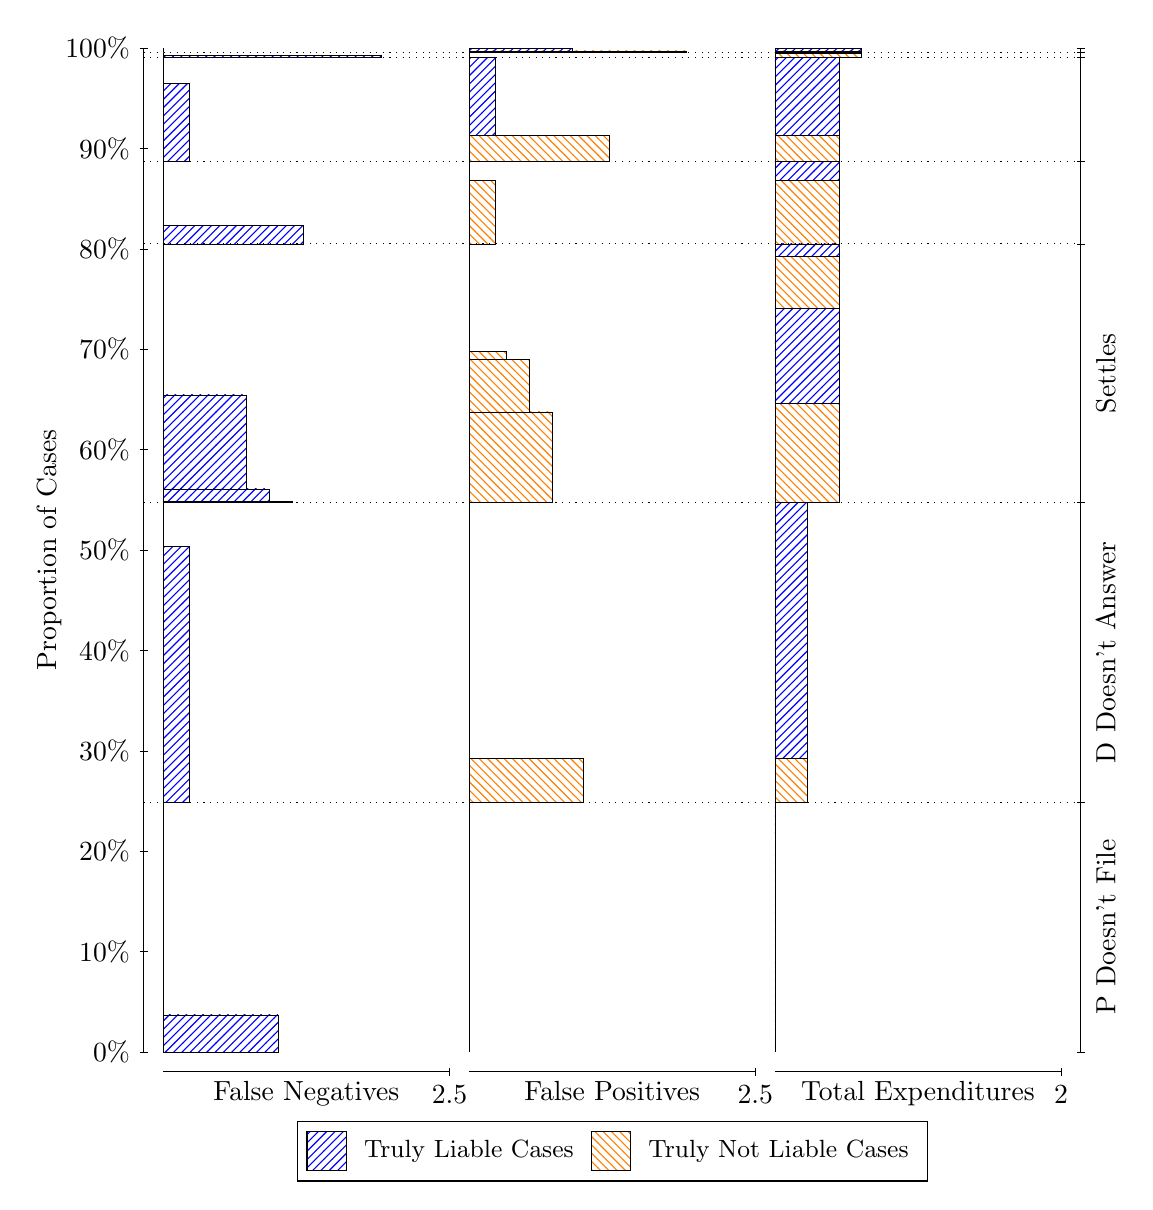
\begin{tikzpicture}
\draw[black, very thin] (1.5,1.75) -- (1.5,14.5);
\node[rotate=90, text=black, anchor=center] at (0.3, 8.125) {Proportion of Cases};
\draw[black, very thin] (1.45,1.75) -- (1.55,1.75);
\node[text=black, anchor=east] at (1.45, 1.75) {0\%};
\draw[black, very thin] (1.45,3.025) -- (1.55,3.025);
\node[text=black, anchor=east] at (1.45, 3.025) {10\%};
\draw[black, very thin] (1.45,4.3) -- (1.55,4.3);
\node[text=black, anchor=east] at (1.45, 4.3) {20\%};
\draw[black, very thin] (1.45,5.575) -- (1.55,5.575);
\node[text=black, anchor=east] at (1.45, 5.575) {30\%};
\draw[black, very thin] (1.45,6.85) -- (1.55,6.85);
\node[text=black, anchor=east] at (1.45, 6.85) {40\%};
\draw[black, very thin] (1.45,8.125) -- (1.55,8.125);
\node[text=black, anchor=east] at (1.45, 8.125) {50\%};
\draw[black, very thin] (1.45,9.4) -- (1.55,9.4);
\node[text=black, anchor=east] at (1.45, 9.4) {60\%};
\draw[black, very thin] (1.45,10.675) -- (1.55,10.675);
\node[text=black, anchor=east] at (1.45, 10.675) {70\%};
\draw[black, very thin] (1.45,11.95) -- (1.55,11.95);
\node[text=black, anchor=east] at (1.45, 11.95) {80\%};
\draw[black, very thin] (1.45,13.225) -- (1.55,13.225);
\node[text=black, anchor=east] at (1.45, 13.225) {90\%};
\draw[black, very thin] (1.45,14.5) -- (1.55,14.5);
\node[text=black, anchor=east] at (1.45, 14.5) {100\%};

\draw[black, very thin] (13.4,1.75) -- (13.4,14.5);
\draw[black, very thin] (13.35,1.75) -- (13.45,1.75);
\node[anchor=west] at (13.35, 1.75) {};
\draw[black, very thin] (13.35,4.9236) -- (13.45,4.9236);
\node[anchor=west] at (13.35, 4.9236) {};
\draw[black, very thin] (13.35,8.7272) -- (13.45,8.7272);
\node[anchor=west] at (13.35, 8.7272) {};
\draw[black, very thin] (13.35,12.014) -- (13.45,12.014);
\node[anchor=west] at (13.35, 12.014) {};
\draw[black, very thin] (13.35,13.057) -- (13.45,13.057);
\node[anchor=west] at (13.35, 13.057) {};
\draw[black, very thin] (13.35,14.383) -- (13.45,14.383);
\node[anchor=west] at (13.35, 14.383) {};
\draw[black, very thin] (13.35,14.446) -- (13.45,14.446);
\node[anchor=west] at (13.35, 14.446) {};
\draw[black, very thin] (13.35,14.5) -- (13.45,14.5);
\node[anchor=west] at (13.35, 14.5) {};

\draw[black, very thin, pattern color=blue, pattern=north east lines] (1.75,1.75) rectangle (3.2033,2.2217);
\draw[black, very thin, pattern color=orange, pattern=north west lines] (1.75,2.2217) rectangle (1.75,4.9236);
\draw[black, very thin, pattern color=blue, pattern=north east lines] (1.75,4.9236) rectangle (2.077,8.1744);
\draw[black, very thin, pattern color=orange, pattern=north west lines] (1.75,8.1744) rectangle (1.75,8.7272);
\draw[black, very thin, pattern color=blue, pattern=north east lines] (1.75,8.7272) rectangle (3.385,8.7417);
\draw[black, very thin, pattern color=blue, pattern=north east lines] (1.75,8.7417) rectangle (3.0943,8.9009);
\draw[black, very thin, pattern color=blue, pattern=north east lines] (1.75,8.9009) rectangle (2.8037,10.094);
\draw[black, very thin, pattern color=orange, pattern=north west lines] (1.75,10.094) rectangle (1.75,12.014);
\draw[black, very thin, pattern color=blue, pattern=north east lines] (1.75,12.014) rectangle (3.5303,12.249);
\draw[black, very thin, pattern color=orange, pattern=north west lines] (1.75,12.249) rectangle (1.75,13.057);
\draw[black, very thin, pattern color=blue, pattern=north east lines] (1.75,13.057) rectangle (2.077,14.053);
\draw[black, very thin, pattern color=orange, pattern=north west lines] (1.75,14.053) rectangle (1.75,14.383);
\draw[black, very thin, pattern color=blue, pattern=north east lines] (1.75,14.383) rectangle (4.5113,14.402);
\draw[black, very thin, pattern color=orange, pattern=north west lines] (1.75,14.402) rectangle (1.75,14.446);
\draw[black, very thin, pattern color=orange, pattern=north west lines] (1.75,14.446) rectangle (1.75,14.465);
\draw[black, very thin, pattern color=blue, pattern=north east lines] (1.75,14.465) rectangle (1.75,14.5);
\draw[black, very thin, pattern color=orange, pattern=north west lines] (5.6333,1.75) rectangle (5.6333,4.4519);
\draw[black, very thin, pattern color=blue, pattern=north east lines] (5.6333,4.4519) rectangle (5.6333,4.9236);
\draw[black, very thin, pattern color=orange, pattern=north west lines] (5.6333,4.9236) rectangle (7.0867,5.4764);
\draw[black, very thin, pattern color=blue, pattern=north east lines] (5.6333,5.4764) rectangle (5.6333,8.7272);
\draw[black, very thin, pattern color=orange, pattern=north west lines] (5.6333,8.7272) rectangle (6.687,9.8785);
\draw[black, very thin, pattern color=orange, pattern=north west lines] (5.6333,9.8785) rectangle (6.3963,10.543);
\draw[black, very thin, pattern color=orange, pattern=north west lines] (5.6333,10.543) rectangle (6.1057,10.647);
\draw[black, very thin, pattern color=blue, pattern=north east lines] (5.6333,10.647) rectangle (5.6333,12.014);
\draw[black, very thin, pattern color=orange, pattern=north west lines] (5.6333,12.014) rectangle (5.9603,12.822);
\draw[black, very thin, pattern color=blue, pattern=north east lines] (5.6333,12.822) rectangle (5.6333,13.057);
\draw[black, very thin, pattern color=orange, pattern=north west lines] (5.6333,13.057) rectangle (7.4137,13.387);
\draw[black, very thin, pattern color=blue, pattern=north east lines] (5.6333,13.387) rectangle (5.9603,14.383);
\draw[black, very thin, pattern color=orange, pattern=north west lines] (5.6333,14.383) rectangle (5.6333,14.427);
\draw[black, very thin, pattern color=blue, pattern=north east lines] (5.6333,14.427) rectangle (5.6333,14.446);
\draw[black, very thin, pattern color=orange, pattern=north west lines] (5.6333,14.446) rectangle (8.3947,14.465);
\draw[black, very thin, pattern color=blue, pattern=north east lines] (5.6333,14.465) rectangle (6.9413,14.5);
\draw[black, very thin, pattern color=orange, pattern=north west lines] (9.5167,1.75) rectangle (9.5167,4.4519);
\draw[black, very thin, pattern color=blue, pattern=north east lines] (9.5167,4.4519) rectangle (9.5167,4.9236);
\draw[black, very thin, pattern color=orange, pattern=north west lines] (9.5167,4.9236) rectangle (9.9254,5.4764);
\draw[black, very thin, pattern color=blue, pattern=north east lines] (9.5167,5.4764) rectangle (9.9254,8.7272);
\draw[black, very thin, pattern color=orange, pattern=north west lines] (9.5167,8.7272) rectangle (10.334,9.9826);
\draw[black, very thin, pattern color=blue, pattern=north east lines] (9.5167,9.9826) rectangle (10.334,11.19);
\draw[black, very thin, pattern color=orange, pattern=north west lines] (9.5167,11.19) rectangle (10.334,11.854);
\draw[black, very thin, pattern color=blue, pattern=north east lines] (9.5167,11.854) rectangle (10.334,12.014);
\draw[black, very thin, pattern color=orange, pattern=north west lines] (9.5167,12.014) rectangle (10.334,12.822);
\draw[black, very thin, pattern color=blue, pattern=north east lines] (9.5167,12.822) rectangle (10.334,13.057);
\draw[black, very thin, pattern color=orange, pattern=north west lines] (9.5167,13.057) rectangle (10.334,13.387);
\draw[black, very thin, pattern color=blue, pattern=north east lines] (9.5167,13.387) rectangle (10.334,14.383);
\draw[black, very thin, pattern color=orange, pattern=north west lines] (9.5167,14.383) rectangle (10.607,14.427);
\draw[black, very thin, pattern color=blue, pattern=north east lines] (9.5167,14.427) rectangle (10.607,14.446);
\draw[black, very thin, pattern color=orange, pattern=north west lines] (9.5167,14.446) rectangle (10.607,14.465);
\draw[black, very thin, pattern color=blue, pattern=north east lines] (9.5167,14.465) rectangle (10.607,14.5);
\draw[black, dotted] (1.5,4.9236) -- (13.4,4.9236);
\draw[black, dotted] (1.5,8.7272) -- (13.4,8.7272);
\draw[black, dotted] (1.5,12.014) -- (13.4,12.014);
\draw[black, dotted] (1.5,13.057) -- (13.4,13.057);
\draw[black, dotted] (1.5,14.383) -- (13.4,14.383);
\draw[black, dotted] (1.5,14.446) -- (13.4,14.446);
\draw[black, very thin] (1.75,1.5) -- (5.3833,1.5);
\node[text=black, anchor=north] at (3.5667, 1.5) {False Negatives};
\draw[black, very thin] (5.3833,1.45) -- (5.3833,1.55);
\node[text=black, anchor=north] at (5.3833, 1.45) {2.5};

\draw[black, very thin] (5.6333,1.5) -- (9.2667,1.5);
\node[text=black, anchor=north] at (7.45, 1.5) {False Positives};
\draw[black, very thin] (9.2667,1.45) -- (9.2667,1.55);
\node[text=black, anchor=north] at (9.2667, 1.45) {2.5};

\draw[black, very thin] (9.5167,1.5) -- (13.15,1.5);
\node[text=black, anchor=north] at (11.333, 1.5) {Total Expenditures};
\draw[black, very thin] (13.15,1.45) -- (13.15,1.55);
\node[text=black, anchor=north] at (13.15, 1.45) {2};

\node[text=black, centered, rotate=90] at (13.72, 3.3368) {P Doesn't File};
\node[text=black, centered, rotate=90] at (13.72, 6.8254) {D Doesn't Answer};
\node[text=black, centered, rotate=90] at (13.72, 10.37) {Settles};





\draw (7.449999999999999,1.5) node[draw=none] (baseCoordinate) {};
\begin{scope}[align=center]
        \matrix[scale=0.5, draw=black, below=0.5cm of baseCoordinate, nodes={draw}, column sep=0.1cm]{
            \node[rectangle, draw, minimum width=0.5cm, minimum height=0.5cm, pattern color=blue, pattern=north east lines] {}; &
            \node[draw=none, font=\small, text=black] (B) {Truly Liable Cases}; &
            \node[rectangle, draw, minimum width=0.5cm, minimum height=0.5cm, pattern color=orange, pattern=north west lines] {}; &
            \node[draw=none, font=\small, text=black] (B) {Truly Not Liable Cases}; \\
            };
\end{scope}

\end{tikzpicture}
\end{document}